\documentclass{article}
\textwidth=6in
\hoffset=0in
\voffset=0in

\usepackage[a4paper, total={6in, 8in}]{geometry}
\usepackage{amsmath}
\usepackage{amssymb}
\usepackage{stmaryrd}
\usepackage{graphicx}
\usepackage{tikz}
\usetikzlibrary{automata, arrows}
\usepackage{pifont}
\usepackage{amssymb}
\usepackage{gensymb}
\usepackage{ngerman}
\usepackage[ampersand]{easylist}

% needs to be updated
\author{Max Springenberg, 177792}
\title{\
    GTI Uebungsblatt 3
    }
\setcounter{section}{3}
\date{}

% custom commands
% \Theta \Omega \omega
\newcommand{\tab}{\null\ \qquad}
\newcommand{\gap}{\null\ \\ \\}
\newcommand{\lA}{\leftarrow}
\newcommand{\rA}{\rightarrow}
\newcommand{\ue}{\infty}
\newcommand{\eps}{\epsilon}
\newcommand{\task}[1]{\textbf{#1} \\ \gap}
\newcommand{\cmark}{\ding{51}}
\newcommand{\xmark}{\ding{55}}
\newcommand{\degr}{\degree}
\newcommand{\LRA}{\Leftrightarrow}
\renewcommand{\~}{\sim}

% content
\begin{document}
% title page
\maketitle
\newpage
% actual paper
\subsection\
1.\\
Das entfernen  aller Zust"ande von $A$, die nicht von $s$ aus erreichbar sind
    resultiert in dem Entfernen von 7 und 8.\\
2.\\
Die daraus resultierende Relation $N(A)$ und die jewiligen Zustandspaare lassen
    sich aus folgender Tabelle ablesen.\\
\begin{tabular}{l|l|l|l|l|l|l}
        &1      &2      &3      &4      &5      &6   \\ 
    \hline
    1   & -     &$x^0$  &$x^2$  &$x^2$  &$x^0$  &     \\
    \hline
    2   & -     & -     &$x^1$  &$x^0$  &$x^1$  &$x^0$\\
    \hline
    3   & -     & -     & -     &$x^0$  &$x^1$  &$x^2$\\
    \hline
    4   & -     & -     & -     & -     &$x^1$  &$x^2$\\
    \hline
    5   & -     & -     & -     & -     & -     &$x^0$\\
    \hline
    6   & -     & -     & -     & -     & -     & -   \\
\end{tabular}\\
3.\\
Das Verschmelzen der nicht markierten Zust"ande liefert den Folgenden 
    Automaten.\\
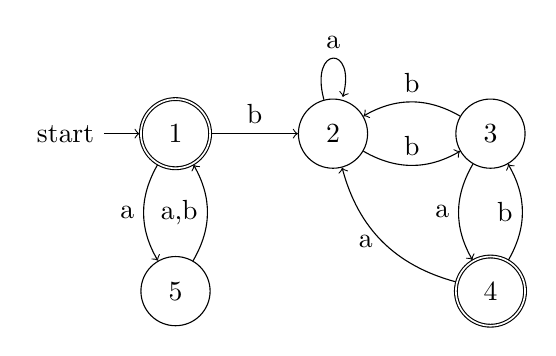
\begin{tikzpicture}
    \node[initial, accepting, state](1) at (0,0) {1};
    \node[state](2)             at (2,0) {2};
    \node[state](3)             at (4,0) {3};
    \node[accepting, state](4)  at (4,-2) {4};
    \node[state](5)             at (0,-2) {5};
    \path
        (1)
            edge [->, bend right, left] node {a} (5)
            edge [->, above] node {b} (2)
        (2)
            edge [->, bend right, above] node {b} (3)
            edge [->, loop above] node {a} (2)
        (3)
            edge [->, bend right, above] node {b} (2)
            edge [->, bend right, left] node {a} (4)
        (4)
            edge [->, bend right, left] node {b} (3)
            edge [->, bend left, left] node {a} (2)
        (5)
            edge [->, bend right, left] node {a,b} (1)
        ;
\end{tikzpicture}\\
\subsection{\
    Sei$
        L = \{ w \in \{a,b\} 
            | |w| > 1 \text{ und der vorletzte Buchstabe in w ist ein b}
            \}
        $
    }
\subsubsection{\
    Geben Sie für jede Äquivalenzklasse der Nerode-Relation $\~_{L}$ einen 
        Repräsentanten an. Geben Sie außerdem für je zwei verschiedene dieser 
        Repräsentanten $x_i$ und $x_j$ ein Wort $z_{ij}$ an, das bezeugt, dass 
        $x_i$ und $x_j$ verschiedene Äquivalenzklassen repräsentieren.
        Es soll also gelten $x_i z_{ij}  \in L \LRA x_j z_ij \in L$ 
        für alle Repräsentanten $x_i, x_j$ mit $x_i \neq x_j$.
    }
M"ogliche Representationen f"ur die "Aquivalenzklassen sind 
    $x_1 = aa, x_2 = ab, x_3 = ba, x_4 = bb$ mit:$\\
    aa \not \~_{L} ab \text{ mit } z = a\\
    ba \not \~_{L} ab \text{ mit } z = \eps\\
    ba \not \~_{L} aa \text{ mit } z = \eps\\
    bb \not \~_{L} aa \text{ mit } z = \eps\\
    bb \not \~_{L} ab \text{ mit } z = \eps\\
    bb \not \~_{L} ba \text{ mit } z = a\\
    $\\
Da dies vier Representationen, zu je einer "Aquivalenzklasse angegeben wurden 
    und nach Aufgabenstellung nur 4 "Aquivalenzklassen existieren, wurde zu 
    jeder "Aquivalenzklasse eine Representation angegeben.\\
\gap
\subsubsection{\
    Geben Sie einen minimalen DFA $A$ an, so dass $L(A) = L$ gilt. Begr"unden 
        Sie sowohl, dass $A$ die Sprache $L$ entscheidet, als auch, dass $A$ 
        minimal ist.
    }
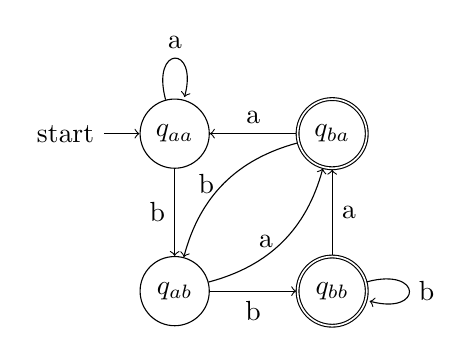
\begin{tikzpicture}
    \node[initial, state](1)    at (0,0) {$q_{aa}$};
    \node[state](2)             at (0,-2) {$q_{ab}$};
    \node[accepting, state](3)  at (2,-2){$q_{bb}$};
    \node[accepting, state](4)  at (2,0){$q_{ba}$};
    \path
        (1)
            edge [->, loop above] node {a} (1)
            edge [->, left] node {b} (2)
        (2)
            edge [->, bend right, left] node {a} (4)
            edge [->, below] node {b} (3)
        (3)
            edge [->, right] node {a} (4)
            edge [->, loop right] node {b} (3)
        (4)
            edge [->, above] node {a} (1)
            edge [->, bend right, left] node {b} (2)
        ;
\end{tikzpicture}\\
$L(A) = L$:\\$
\\
L(A) \subseteq L:\\
\text{Annahme } L(A) \not \subseteq L \text{, dann } 
    \exists w \in L(A) : w \not \in L\\
\\
$ Alle W"orter $w \in L(A)$ sind l"anger als 1, da es mindestens 2 Transitionen
    bedarf um in einen akzeptierenden Zustand zu wechseln. Des weiteren gilt,
    dass alle W"orter genau dann akzeptiert werden, wenn die vorletzte 
    Transition nach einlesen aller Zeichen, durch ein b erfolgte.\\
1. Fall $|w| \leq 1$:\\
$w \not \in L(A) \land w \not \in L$\\
2. Fall $w = va\sigma, v \in \{a,b\}^*, \sigma \in \{a,b\}$:\\
$w \not \in L(A) \land w \not \in L\\
\lightning$ es muss gelten $L(A) \subseteq L$\\
\gap
$L \subseteq L(A):\\
\text{Annahme } L \not \subseteq L(A) \text{, dann } 
    \exists w \in L : w \not \in L(A)\\
\\
$ Alle W"orter aus L sind definiert als l"anger als 1 und mit einem b als
    vorletztes Zeichen.\\
1. Fall $|w| \leq 1$:\\
W"orter aus $L(A)$ muessen l"anger als 1 sein, da es mindestens zwei 
    Transitionen bedarf um in einen akzeptierenden Zustand zu wechseln.\\
$w \not \in L \land w \not \in L(A)$\\
2. Fall $w = va\sigma, v \in \{a,b\}^*, \sigma \in \{a,b\}$:\\
Es wird nur in einen akzeptierenden Zustand gewechselt, wenn die Vorletzte
    Transition durch ein b erfolgte.\\
$w \not \in L(A) \land w \not \in L\\
\lightning$ es muss gelten $L \subseteq L(A)$\\
\\
Damit muss dann auch gelten $L(A) = L$\\
\gap
Ein minimaler DFA hat soviele Zust"ande, wie "Aquivalenzklassen zu der Nerode 
    Relation, der durch diesen entschiedene Sprache existieren. 
    $A$ hat vier Zust"ande und es wurde gezeigt, dass $L(A) = L$ gilt 
    und dass L vier "Aquivalenzklassen enthaelt. Damit ist $A$ minimal.\\
\ \\
\subsection\
\subsubsection\
Der Produktautomat $A$ mit den Akzeptierenden Zust"anden \[ 
    F_A = \{(p,q) \in Q_S \times Q_P 
        | (q \in F_S \land p \not \in F_P)
        \lor (q \not \in F_S \land p \in F_P)\}
    \]
ergibt sich zu:\\
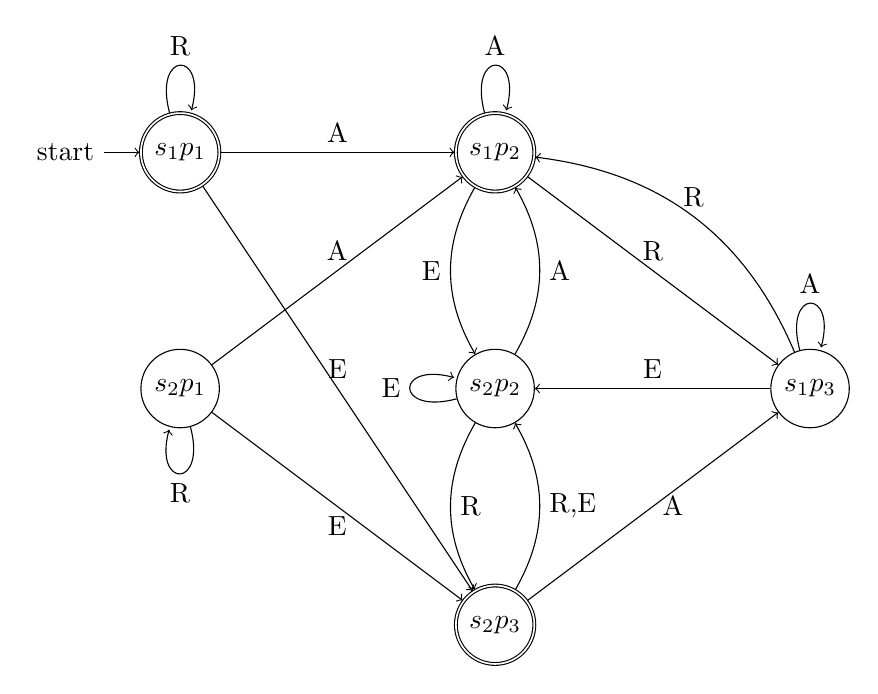
\begin{tikzpicture}
    \node[initial, accepting, state]    (s1p1)  at (0,0) {$s_1 p_1$};
    \node[accepting, state]             (s1p2)  at (4,0) {$s_1 p_2$};
    \node[state]                        (s1p3)  at (8,-3){$s_1 p_3$};
    \node[state]                        (s2p1)  at (0,-3){$s_2 p_1$};
    \node[state]                        (s2p2)  at (4,-3){$s_2 p_2$};
    \node[accepting, state]             (s2p3)  at (4,-6){$s_2 p_3$};
    \path
        (s1p1)
            edge [->, loop above] node {R} (s1p1)
            edge [->, above] node {A} (s1p2)
            edge [->, above] node {E} (s2p3)
        (s1p2)
            edge [->, loop above] node {A} (s1p2)
            edge [->, above] node {R} (s1p3)
            edge [->, bend right, left] node {E} (s2p2)
        (s1p3)
            edge [->, loop above] node {A} (s1p3)
            edge [->, bend right, above] node {R} (s1p2)
            edge [->, above] node {E} (s2p2)
        (s2p1)
            edge [->, loop below] node {R} (s2p1)
            edge [->, above] node {A} (s1p2)
            edge [->, below] node {E} (s2p3)
        (s2p2)
            edge [->, bend right, right] node {A} (s1p2)
            edge [->, bend right, right] node {R} (s2p3)
            edge [->, loop left] node {E} (s2p2)
        (s2p3)
            edge [->, right] node {A} (s1p3)
            edge [->, bend right, right] node {R,E} (s2p2)
        ;
\end{tikzpicture}\\
Ohne den unerreichbaren Zustand $s_2 p_1$:\\
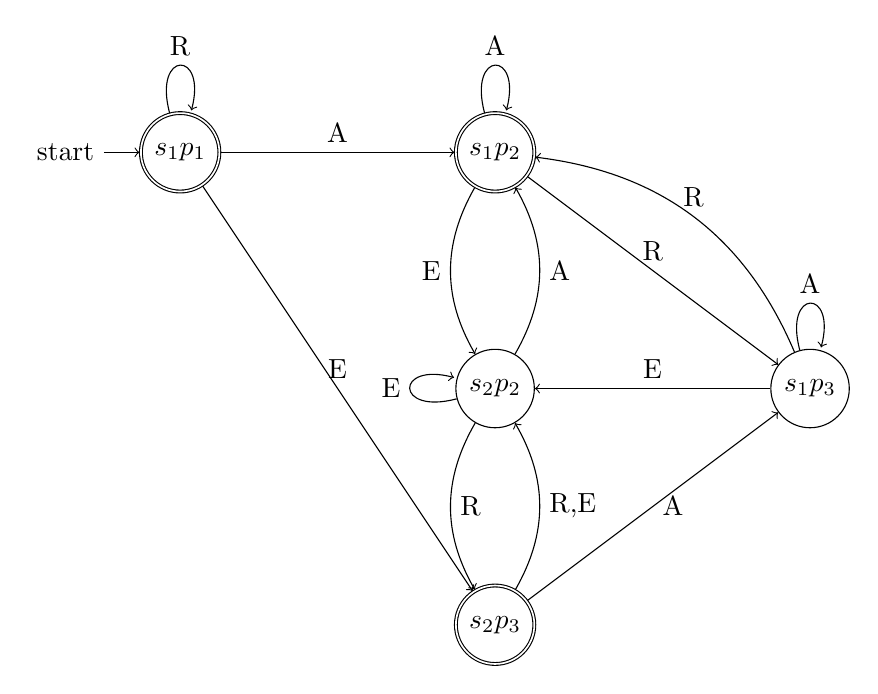
\begin{tikzpicture}
    \node[initial, accepting, state]    (s1p1)  at (0,0) {$s_1 p_1$};
    \node[accepting, state]             (s1p2)  at (4,0) {$s_1 p_2$};
    \node[state]                        (s1p3)  at (8,-3){$s_1 p_3$};
    \node[state]                        (s2p2)  at (4,-3){$s_2 p_2$};
    \node[accepting, state]             (s2p3)  at (4,-6){$s_2 p_3$};
    \path
        (s1p1)
            edge [->, loop above] node {R} (s1p1)
            edge [->, above] node {A} (s1p2)
            edge [->, above] node {E} (s2p3)
        (s1p2)
            edge [->, loop above] node {A} (s1p2)
            edge [->, above] node {R} (s1p3)
            edge [->, bend right, left] node {E} (s2p2)
        (s1p3)
            edge [->, loop above] node {A} (s1p3)
            edge [->, bend right, above] node {R} (s1p2)
            edge [->, above] node {E} (s2p2)
        (s2p2)
            edge [->, bend right, right] node {A} (s1p2)
            edge [->, bend right, right] node {R} (s2p3)
            edge [->, loop left] node {E} (s2p2)
        (s2p3)
            edge [->, right] node {A} (s1p3)
            edge [->, bend right, right] node {R,E} (s2p2)
        ;
\end{tikzpicture}\\
\subsubsection\
Die Sprache $L(A)$ ist nicht leer, damit sind die Automaten nach dem 
    "Aquivalenztest der Vorlesung "uber einen Produktautomaten mit akzeptierenden
    Zust"anden bei zusammen gedassten Zust"anden mit ungleicher 
    Akzeptiereigenschaft nicht "aquivalent.\\
\gap
Ferner erf"ullt $P$ damit auch nicht die Spezifikation $S$.\\
\subsubsection\
Es bietet sich, wie auch in den vorhergehenden Teilaufgaben die Konstruktion
    eines Produktautomaten und ein Leerheitstest f"ur diesen an.\\
\\
Wie in der Vorlesung vorgestellt existiert ein Algorithmus f"ur den 
    Leerheitstest mit:\\
\begin{easylist}
    & Vergiss die Kantenmarkierung 
    & F"uge einen Zielknoten t und f"ur jeden akzeptierenden Zustand eine 
        Transition zu t hinzu.
    & Teste, ob ein Weg von s noch t existiert
    & Wenn ja, so gilt $L(A) \neq \emptyset$
\end{easylist}\ \\
In der Laufzeit $O(|\delta|)$
\\
Die Konstruktion eines Produktautomaten $A$ aus den Automaten $A_1, A_2$ kann 
    durch $A = A_1 \times A_2$ mit \[
    F_A = \{
        (p,q) \in Q_1 \times Q_2 
            | (q \in F_1 \land p \not \in F_2)
            \lor (q \not \in F_1 \land p \in F_2)
        \}
    \]
Nach vorlesung bel"auft sich diese Konstruktion in ihrer Laufzeit auf
    $O(|Q_1| \times |Q_2| \times |\Sigma|)$\\
\\
Der Algorithmus umfasst diese Konstruktion gefolgt von dem Leerheitstest und
    bel"auft dementsprechend auf eine Laufzeit von \[
    O(|Q_1| \times |Q_2| \times |\Sigma| + |\delta|) 
        = O(|Q_1| \times |Q_2| \times |\Sigma|)
    \]
\subsubsection\
Zun"achst wandelt man jeden RA $\alpha_i$ in einen $\eps-NFA$ um, mit dem 
    Baukastenprinzip bel"auft sich das auf $O(|\alpha_i|)$\\
Im folgendem wird der Produktautomat mit durch die $\eps-NFA$s konstruiert
    und deer Leerheitstest berechnet.\\
Da $O(|\alpha|)$ linear ist bleibt die Laufzeit bei \[
    O(|Q_1| \times |Q_2| \times |\Sigma|)
    \]
%\subsection\
%\subsubsection\
%$PRIM$ sei die Menge der Primzahlen.\\
%$L=\{a^n | n \not \equiv_{pq} 1336\}, p,q \in PRIM: p,q < 1336 < pq$\\
%\\
%Gesucht NFA mit $p+q+1$ Zust"anden.\\
%Ein naiver Ansatz w"are es fuer jeden Rest von $\equiv_{pq}$ einen Zustand zu
%    waehlen, da aber nach Aufgabenstellung $p,q<1336<pq$ gilt folgt, dass
%    $p,q$ ungleich $2,3$ sein m"ussen und damit fuer alle F"alle gilt
%    $pq > p+q+1$\\
%Es muss also ein effizienterer Weg gefunden werden.\\
%\\
%\subsubsection\
\end{document}
